\chapter{Legal and Compliance}

\section*{Why This Matters}

Legal and compliance applications represent domains where transformer models address document-intensive workflows with stringent accuracy and explainability requirements fundamentally different from general-purpose AI. These requirements create unique technical and operational challenges. Contract review consumes 30--50\% of associate attorney time. Regulatory compliance requires continuous analysis of evolving regulations across multiple jurisdictions. Legal research involves synthesizing information from millions of case documents. Due diligence in mergers and acquisitions must review thousands of contracts and financial documents within compressed timelines. Financial compliance includes monitoring transactions for suspicious activity and sanctions violations.

Transformer-based systems demonstrate measurable impact: reducing contract review time by 40--60\%, identifying compliance risks with 85--95\% accuracy, and accelerating legal research by 3--5\times. However, success in these domains is determined not by model accuracy alone but by explainability, professional responsibility compliance, integration with existing workflows, and robust quality assurance.

Understanding legal AI applications requires recognizing constraints that distinguish this domain. Explainability requirements where decisions must be justified with specific citations to source documents. Liability considerations where errors can result in multi-million dollar consequences. Professional responsibility standards that maintain attorney oversight and ultimate responsibility for work product. These constraints fundamentally shape technical architecture decisions and deployment strategies.

This chapter examines legal and compliance applications from an engineering perspective, focusing on the technical requirements, explainability constraints, and risk management considerations that determine successful deployment in these high-stakes professional domains.

\section{Contract Analysis and Review}

\begin{figure}[htbp]
\centering
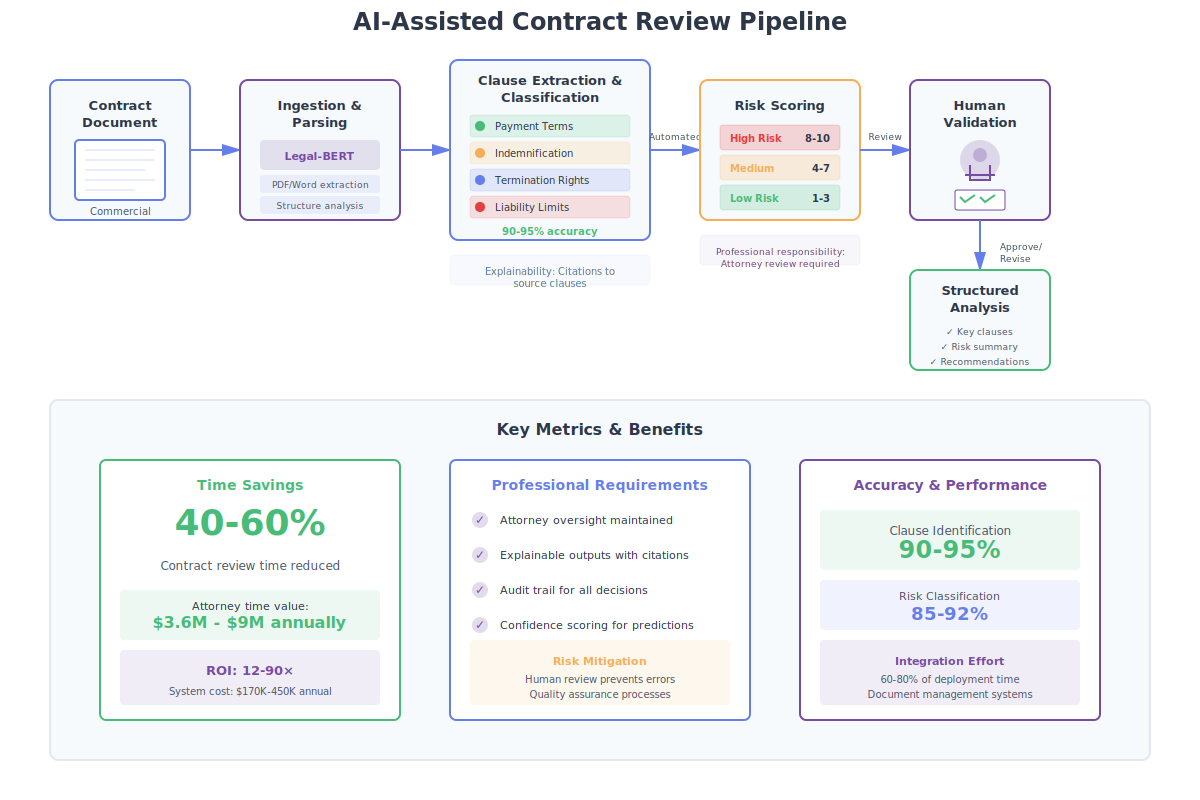
\includegraphics[width=0.95\textwidth]{chapters/diagrams/chapter13_contract_review_a1b2c3d4.png}
\caption{AI-assisted contract review pipeline showing the complete workflow from document ingestion through Legal-BERT processing, clause extraction and classification, risk scoring, attorney validation, and structured analysis output. The system achieves 90-95\% accuracy for clause identification and provides 40-60\% time savings with 12-90× ROI while maintaining required attorney oversight.}
\label{fig:contract_review_pipeline}
\end{figure}

\subsection{Contract Document Characteristics}

Legal contracts differ from general documents in ways that affect model architecture and training strategies. Contracts contain highly structured language with specific legal terminology, defined terms that carry precise meanings within the document, and cross-references creating complex dependency relationships. A single contract might reference dozens of defined terms, each requiring consistent interpretation throughout.

Clause identification and classification require understanding legal concepts and document structure. Standard clauses---indemnification, limitation of liability, termination rights---appear with variations across contracts. Models must recognize semantic equivalence despite syntactic differences: ``Party A shall indemnify Party B'' and ``Party B shall be held harmless by Party A'' express similar obligations despite different wording.

Temporal and conditional logic pervades contract language. Obligations often depend on specific conditions, dates, or events: ``If Party A fails to deliver within 30 days, Party B may terminate.'' Understanding these dependencies requires parsing complex conditional structures and tracking temporal relationships across multiple clauses. Errors in temporal reasoning lead to misidentifying obligations or missing critical deadlines.

Ambiguity detection represents a critical capability for contract review. Vague terms like ``reasonable efforts,'' ``material breach,'' or ``commercially reasonable'' create interpretation risks. Models must identify potentially ambiguous language and flag it for attorney review, as ambiguity often becomes the subject of disputes. This requires understanding not just what text says, but what it fails to specify clearly.

\subsection{Contract Review Models and Approaches}

Specialized legal language models address domain-specific challenges through pre-training on legal corpora. Legal-BERT, trained on 12 GB of legal text from case law, contracts, and statutes, achieves 5--8\% better performance on legal NLP tasks than general BERT. This improvement translates to thousands of correctly identified clauses and obligations in production deployment.

Contract-specific models like ContractBERT focus on contract language patterns, training on millions of commercial contracts. These models learn to recognize standard clause types, identify unusual provisions, and detect missing clauses that typically appear in specific contract types. A model trained on employment contracts learns that non-compete clauses, confidentiality provisions, and termination conditions typically appear together.

Model size for legal applications typically ranges from 110 million to 340 million parameters (BERT-base to BERT-large). Larger models provide better performance on complex legal reasoning tasks but face deployment constraints in law firm IT environments. Many legal organizations lack GPU infrastructure, making efficient models running on CPU more practical despite lower absolute performance.

Fine-tuning legal models requires labeled legal data annotated by legal experts. Attorneys annotating training examples cost \$200--500 per hour depending on specialization. Annotating 10,000 contract clauses costs \$200,000--800,000. This annotation cost often exceeds model training costs, making data efficiency and transfer learning critical for economic viability.

\subsection{Contract Analysis Applications}

Clause extraction and classification identify and categorize contract provisions. Models extract key clauses---payment terms, delivery obligations, warranties, indemnification---and classify them by type and risk level. This extraction enables automated contract analysis, comparison, and risk assessment at scale.

Implementation requires high accuracy thresholds. Missing a critical indemnification clause or misclassifying a limitation of liability provision exposes organizations to significant financial risk. Typical accuracy targets: 90--95\% for standard clause identification, with attorney review of all flagged items. The system reduces review time while maintaining quality through human oversight.

Risk identification systems analyze contracts for provisions deviating from standard terms or creating unusual obligations. Models flag unlimited liability provisions, unusual termination rights, or missing force majeure clauses. These systems learn risk patterns from historical contracts and attorney feedback, improving over time.

Contract comparison enables analysis of multiple versions or similar agreements. Models identify differences between contract versions, highlight non-standard provisions compared to templates, and detect inconsistencies across related agreements. This capability accelerates contract negotiation by quickly identifying changes and implications.

Obligation extraction identifies commitments, deadlines, and deliverables from contracts. Models extract structured information: who must do what, by when, under what conditions. This extraction enables automated contract management, deadline tracking, and compliance monitoring.

\subsection{Contract Performance and Lifecycle Management}

Post-signature contract management ensures organizations track and comply with obligations. Obligation tracking systems identify payment deadlines, delivery dates, renewal dates, and reporting requirements. Automated alerts notify relevant parties of upcoming obligations.

Breach detection identifies when parties fail to meet obligations. The system monitors performance data, transactions, or event logs to determine if obligations are being met. Real-time alerts enable rapid response to breaches.

Renewal and expiration tracking ensures contracts renew appropriately or terminate intentionally rather than through inadvertent lapse. This prevents unintended contract continuations and ensures intentional renegotiation of critical agreements.

Renegotiation identification signals when contracts should be renegotiated based on performance, changing business conditions, or market conditions. Models can identify when terms have become unfavorable and recommend renegotiation, or identify contracts whose terms approach expiration.

\section{Merger and Acquisition Due Diligence}

\begin{figure}[htbp]
\centering
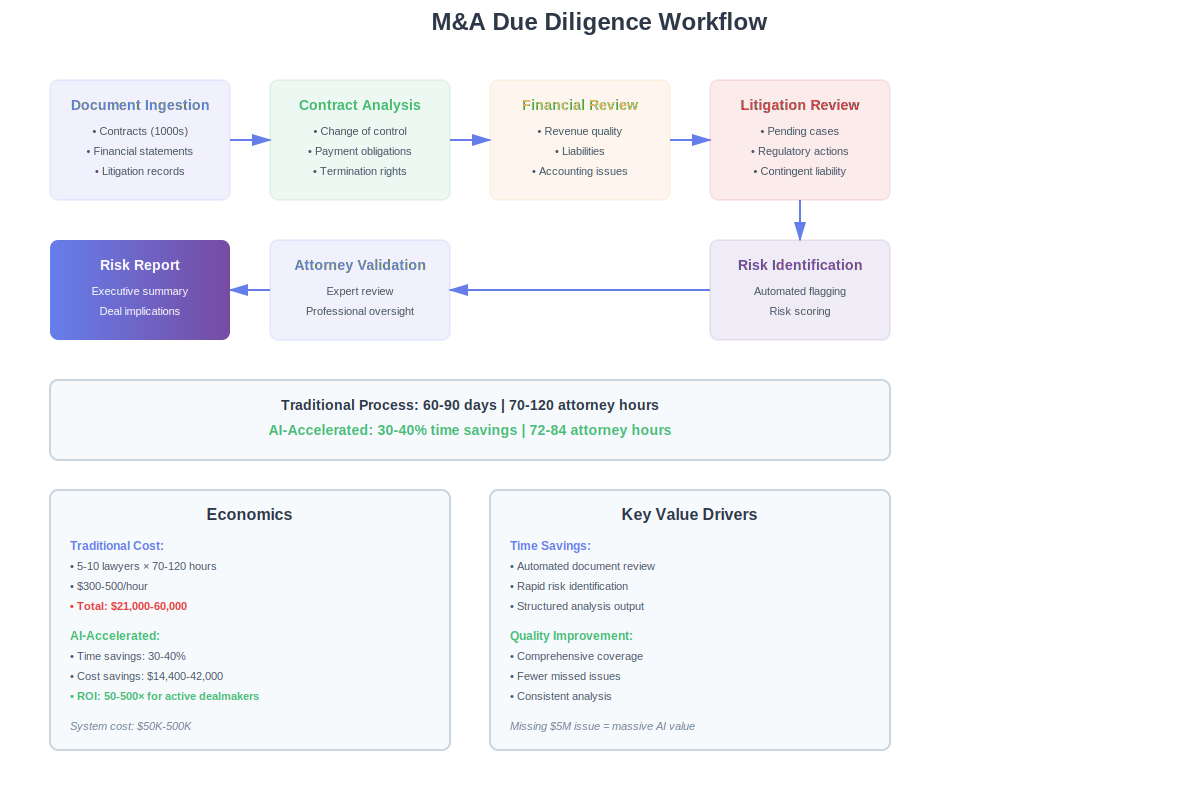
\includegraphics[width=0.95\textwidth]{chapters/diagrams/chapter13_due_diligence_q1r2s3t4.png}
\caption{AI-assisted M\&A due diligence workflow showing document ingestion, contract portfolio analysis, financial statement review, litigation and contingent liability identification, and risk reporting. The system accelerates due diligence by 30--40\%, reducing attorney hours from 120 to 72--84 hours per transaction, with ROI reaching 50--500× for active dealmakers.}
\label{fig:due_diligence_workflow}
\end{figure}

\subsection{Due Diligence Process and Requirements}

M\&A due diligence investigates target companies before acquisition, identifying risks that affect deal price and post-acquisition integration. The process is time-critical---most transactions require completion within 60--90 days---and document-intensive, requiring review of thousands of contracts, financial statements, litigation records, and regulatory filings.

Financial due diligence reviews target company financial statements, identifying risks: undisclosed liabilities, revenue quality issues, accounting irregularities. Regulatory compliance due diligence identifies exposure to regulatory violations, pending enforcement actions, or compliance gaps. Contract and obligation analysis identifies commitments that will transfer to acquirer, including unusual or onerous terms.

Litigation and contingent liability review identifies potential legal exposure: pending litigation, regulatory investigations, product liability risks, environmental liabilities. Missing one material liability can affect deal economics by millions of dollars.

Environmental and compliance due diligence assesses exposure to environmental liabilities, occupational safety issues, and industry-specific regulations. Costs of environmental remediation, regulatory cleanup, or compliance improvements can be substantial.

Intellectual property portfolio review identifies patent, trademark, and trade secret assets; assesses infringement risks; and evaluates freedom to operate in key markets.

\subsection{AI-Assisted Due Diligence}

AI systems accelerate due diligence by automating document review and risk identification. The process typically involves: document ingestion and classification, contract and financial analysis, risk identification and flagging, executive summary generation, and attorney validation.

Contract portfolio analysis identifies key terms: payment obligations, renewal dates, termination conditions, change of control provisions. Many acquisition agreements include change of control clauses triggering events at acquisition (early termination, consent requirements, renegotiation), creating significant risk if missed. Models scan contracts to identify these clauses and highlight implications.

Financial statement analysis identifies risks in financial data: unusual revenue recognition, significant write-downs, contingent liabilities. While AI cannot perform full financial audits, it can flag patterns for accountant attention.

Litigation and contingent liability review scans legal documents, litigation records, and regulatory filings to identify potential exposure. Models identify cases involving the target company, regulatory investigations, and settlement agreements.

\subsection{Economic Impact and Feasibility}

Due diligence traditionally requires weeks of attorney and specialist time. A typical mid-market acquisition involves 5--10 lawyers spending 40--60 hours on contract review, 10--20 hours on compliance analysis, 20--40 hours on litigation/contingent liability. Total effort: 70--120 lawyer-hours at \$300--500 per hour = \$21,000--60,000.

AI acceleration of due diligence has two value components: time savings and quality improvement. Time savings of 30--40\% reduce attorney hours from 120 to 72--84 hours, saving \$14,400--42,000 per transaction. Quality improvement (fewer missed issues) is harder to quantify but potentially more valuable. Missing a material issue that later costs \$5 million represents massive value from AI that prevents the miss.

Deployment cost for due diligence systems ranges from \$50,000 to \$500,000 depending on customization and scope. At that cost, systems become profitable after 5--10 transactions. For active dealmakers, ROI reaches 50--500\times annually.

\section{Financial Compliance and Anti-Money Laundering}

\begin{figure}[htbp]
\centering
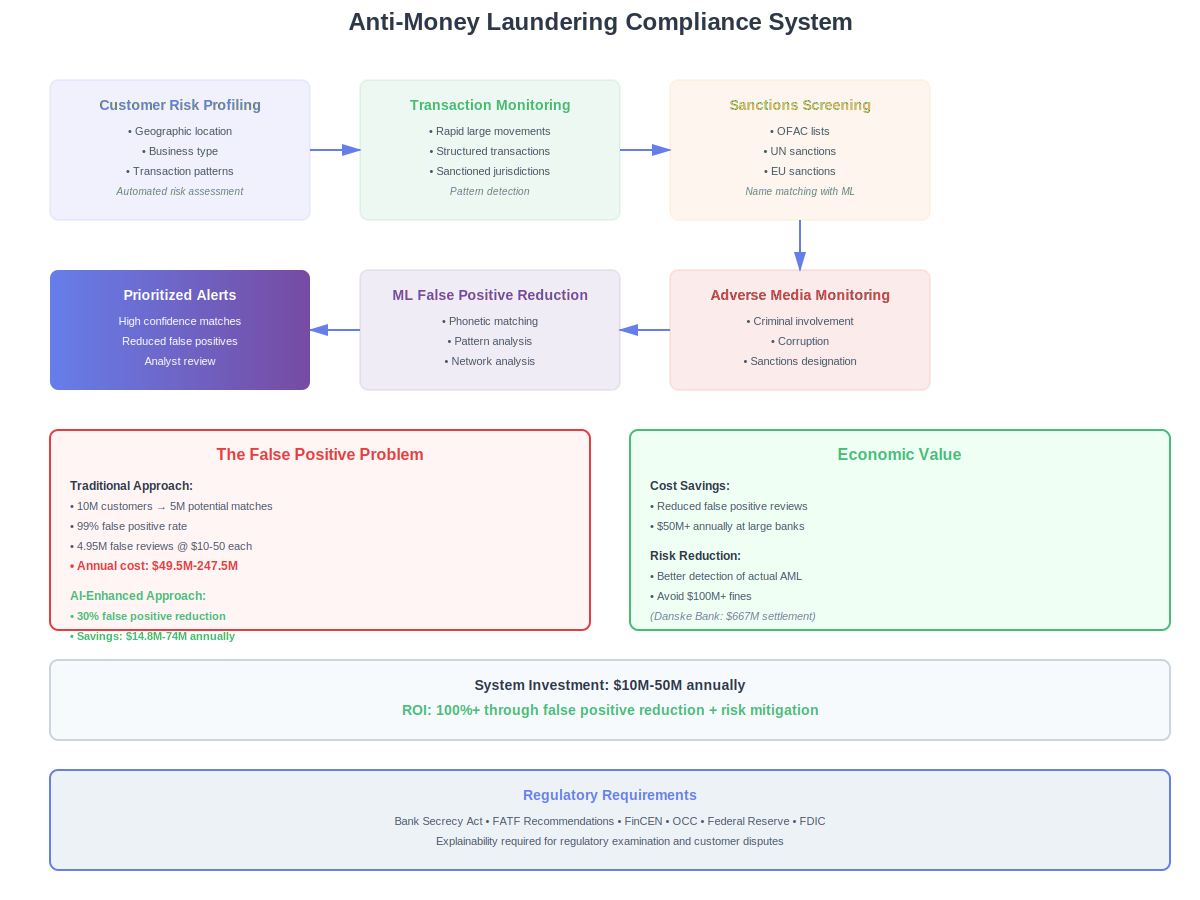
\includegraphics[width=0.95\textwidth]{chapters/diagrams/chapter13_aml_compliance_u5v6w7x8.png}
\caption{Anti-money laundering compliance system showing customer risk profiling, transaction monitoring, sanctions screening, and adverse media monitoring. The system reduces false positive alerts by 30\%, saving \$14.8--74 million annually at large institutions while improving detection of actual suspicious activity.}
\label{fig:aml_compliance_system}
\end{figure}

\subsection{Anti-Money Laundering and Sanctions Compliance}

Financial institutions are required by law (Bank Secrecy Act, FATF recommendations) to prevent use of their systems for money laundering and terrorism financing. This requires customer due diligence at account opening, ongoing transaction monitoring, and suspicious activity reporting.

Customer risk profiling at account opening assesses risk based on customer characteristics: geographic location, business type, transaction patterns. High-risk customers require enhanced due diligence. Models assess risk automatically, applying regulatory rules and learned patterns from historical data. A customer establishing accounts through shell companies in high-risk jurisdictions triggers heightened scrutiny.

Transaction monitoring detects suspicious patterns: rapid movement of large sums, round-dollar transactions, structured transactions designed to evade reporting thresholds, transfers to sanctioned jurisdictions. Models learn normal patterns for customer types and flag deviations. A customer normally moving \$10,000 weekly but suddenly moving \$500,000 in single transactions triggers investigation.

Sanctions screening verifies customers and counterparties against sanctions lists (OFAC, UN, EU, jurisdiction-specific lists). Automated screening compares customer names against sanctions lists, with manual review of matches to avoid false positives. Name matching is challenging due to variations: John Smith vs. John T. Smith vs. J. Smith.

Adverse media monitoring tracks public news and information about customers and counterparties for negative information: criminal involvement, corruption, sanctions designation, bankruptcy. Models ingest news and financial data, identifying relevant adverse information.

\subsection{False Positive Problem and AI Solutions}

A major pain point in financial compliance is false positive alerts. A customer named Mohammad Hussein matching ``Mohammad Hussein'' on a terrorism watch list generates an alert, even though it's a common name. Banks receive millions of potential matches, most of which are false positives requiring manual review.

Each manual review costs approximately \$10--50 depending on complexity. For a bank with 10 million customers generating 5 million potential matches annually with 99\% false positive rate: 4.95 million false reviews cost \$49.5--247.5 million annually. Reducing false positives by 30\% saves \$14.8--74 million annually.

Machine learning models learn patterns distinguishing false positives from true positives. Name matching can consider soundex/phonetic similarity, transaction pattern matching, and network analysis. A ``Mohammad Hussein'' with normal transaction patterns and no adverse information is likely false positive. A ``Mohammad Hussein'' with suspicious transaction patterns, offshore accounts, and adverse media coverage is higher risk.

\subsection{Regulatory Drivers and Economic Value}

Regulatory agencies (FinCEN, OCC, Federal Reserve, FDIC) impose strict requirements and substantial penalties for compliance failures. A bank with inadequate AML controls faces fines of \$100 million+. The Danske Bank Latvia case resulted in \$667 million settlement. Compliance failure creates catastrophic risk.

The economic value of AI in AML is twofold: cost savings from reducing false positives and risk reduction from better detection. Cost savings of \$50 million annually at large institutions justify \$10--50 million annual system investment. Risk reduction of even 1\% improvement in catching actual money laundering saves tens of millions in avoided fines and remediation.

\subsection{Implementation Challenges}

AML systems must integrate with core banking platforms, transaction systems, and customer data systems. Integration complexity is substantial due to diverse legacy systems and regulatory requirements for audit trails and documentation. A bank might have 20+ systems requiring integration.

Tuning and optimization is essential. Model thresholds for alerts must balance detection (catching bad activity) against false positive burden. A threshold that catches 99\% of suspicious activity might generate 5 million false alerts; a threshold generating 1 million false alerts might miss significant activity. Finding the right balance requires continuous tuning based on analyst feedback.

Explainability is required for regulatory examination and customer disputes. When an account is blocked on AML grounds, the institution must explain why. Models must provide reasoning: which sanctions list triggered the match, which transaction patterns were suspicious, which adverse information was found.

\section{Regulatory Compliance and Risk Monitoring}

\subsection{Regulatory Text Characteristics}

Regulatory documents present unique challenges for NLP. Regulations span multiple jurisdictions with different legal frameworks, evolve continuously through amendments and new rulings, and contain complex cross-references. A single regulation might reference dozens of other regulatory provisions, statutes, and guidance documents.

Regulatory language combines prescriptive requirements with interpretive guidance. Some provisions specify exact requirements: ``must maintain records for seven years.'' Others provide principles-based guidance: ``implement appropriate safeguards.'' Models must distinguish mandatory requirements from recommended practices, as compliance obligations differ fundamentally.

Applicability determination requires understanding which regulations apply to specific organizations. A financial services firm might be subject to SEC regulations, state banking laws, international standards like Basel III, and jurisdiction-specific requirements. Models must determine applicability based on organization characteristics, business activities, and geographic scope.

Change detection and impact analysis represent critical capabilities. When regulations change, organizations must identify affected policies, procedures, and controls. Models must detect regulatory changes, assess their significance, and map them to internal compliance frameworks.

\subsection{Specialized Compliance Domains}

Healthcare compliance includes HIPAA, anti-kickback statutes, Stark law prohibitions on self-referral, and fraud and abuse regulations. Each requires different monitoring and documentation.

Environmental compliance includes EPA Clean Air and Water Act regulations, state environmental requirements, emissions reporting. Organizations managing hazardous materials or operating in sensitive environments face complex requirements.

Labor law compliance includes wage and hour requirements, workplace safety (OSHA), anti-discrimination laws. Employment practices must comply with evolving regulatory requirements.

Export control and sanctions compliance includes OFAC sanctions, EAR controls, ITAR restrictions. Organizations exporting goods or services must navigate complex international regulations.

Tax compliance includes transfer pricing documentation, tax reporting requirements, FATCA and CRS requirements. Tax regulations are complex and jurisdiction-dependent.

Product safety and recall regulations vary by industry and product type. Consumer products must comply with CPSC requirements; medical devices with FDA; pharmaceuticals with FDA.

\subsection{Compliance Monitoring Systems}

Regulatory monitoring systems track regulatory changes and assess their impact. These systems ingest regulatory updates from multiple sources and analyze them for relevance and impact.

Architecture typically combines document ingestion, change detection, relevance classification, and impact assessment. Natural language understanding enables automated relevance determination. Models analyze regulatory text to identify applicable industries, activities, and jurisdictions.

Entity and obligation extraction identifies regulatory requirements. Models extract: what must be done, by whom, by when, with what documentation. This structured extraction enables comparison with existing policies and identification of compliance gaps.

Risk scoring assesses compliance risk based on regulatory requirements, organizational controls, and violation history. Models analyze the gap between regulatory requirements and implemented controls.

Explainability is critical. Compliance officers must understand why the system flagged a requirement, which regulations are affected, and what evidence supports the assessment.

\subsection{Continuous Monitoring and Reporting}

Deployed compliance systems must continuously monitor for violations. Models analyze operational data---transaction logs, access records, system configurations---for compliance violations or risk indicators.

Regulatory reporting automates the process of generating required reports. Models extract relevant data, format it according to regulatory specifications, and generate submission-ready documents.

Audit support provides evidence and documentation for regulatory examinations. Models maintain detailed logs of monitoring, decisions, and actions, enabling rapid production of audit evidence.

\section{Legal Research and E-Discovery}

\subsection{Case Law Analysis and Legal Research}

Legal research involves analyzing vast corpora of case law, statutes, and legal commentary to find relevant precedents. Traditional research requires manually searching and reviewing hundreds or thousands of documents. Transformer-based systems accelerate this through semantic search, relevance ranking, and automated summarization.

Semantic search enables finding relevant cases based on legal concepts rather than keyword matching. An attorney searching for ``duty of care in autonomous vehicle accidents'' should find relevant cases even if they use different terminology. Models trained on legal text learn to recognize semantic equivalence across different phrasings of legal concepts.

Citation analysis reveals precedential relationships. Models analyze citation networks to identify influential cases, track how legal doctrines evolve, and assess the strength of legal arguments. A case cited by hundreds of subsequent decisions carries more precedential weight than one rarely cited.

Multi-document synthesis combines information from multiple sources to answer legal questions. A model might synthesize holdings from dozens of cases to identify the prevailing rule in a jurisdiction. This synthesis requires understanding legal reasoning and identifying consistent patterns.

Automated summarization reduces time attorneys spend reading lengthy opinions. Models generate summaries highlighting the key holdings and reasoning. Extractive summarization selects important sentences; abstractive summarization generates new text capturing key points.

\subsection{E-Discovery and Document Review}

E-discovery involves reviewing massive document collections to identify responsive materials for litigation. Document volumes in complex litigation reach millions, making manual review prohibitively expensive. Technology-assisted review (TAR) using machine learning reduces review costs by 40--70\%.

Predictive coding trains models on attorney-reviewed documents. Attorneys review a seed set, labeling documents as relevant or not. Models learn from these labels and predict relevance for remaining documents. Continuous active learning improves model performance iteratively by selecting documents for attorney review that will most improve accuracy.

Statistical validation ensures the review process is reliable. Courts require demonstrating that TAR achieved target recall (finding responsive documents) and precision. Models must achieve 75--85\% recall with measurable precision. This requires statistical sampling and validation throughout the review process.

Privilege review identifies attorney-client privileged communications that must be withheld. This requires understanding privilege concepts, recognizing attorney-client relationships, and identifying legal advice. Errors waive privilege, exposing confidential communications. Typical approach: models flag potential privilege documents for attorney review rather than making final determinations.

Class action discovery involves millions of documents across thousands of parties. Class actions require managing complexity of multiple plaintiffs, defendants, and relevant parties. E-discovery in class actions is particularly expensive and demanding.

\subsection{Litigation Risk and Outcome Prediction}

Early litigation risk prediction assesses which disputes are likely to escalate to litigation. Models trained on dispute history predict likelihood of litigation based on dispute characteristics. Early identification enables settlement discussions before litigation becomes inevitable.

Case outcome prediction estimates likelihood of winning or losing based on facts and law. Models learn from historical case outcomes, identifying patterns that correlate with success. While not perfect, case outcome prediction improves settlement negotiations by enabling realistic assessment of case value.

Damages estimation enables negotiating appropriate settlements. Models estimate likely damages based on case facts, comparable cases, and judicial patterns. Better estimates of case value enable more rational settlement.

Settlement prediction identifies disputes likely to settle and optimal settlement ranges. This enables focusing litigation resources on cases unlikely to settle while pursuing settlement discussions where settlement is probable.

\section{Patent and Intellectual Property}

\subsection{Patent Classification and Prior Art Search}

Patent classification and analysis helps organizations manage patent portfolios and assess IP strategy. Models classify patents by technology domain, identify relevant patents in prior art searches, and assess patent portfolio strength.

Prior art search identifies existing patents that anticipate or render obvious patent applications. Traditional prior art search by specialists costs \$5,000--20,000. Automated search reduces cost and improves comprehensiveness. Models trained on patent corpora can identify relevant prior art more systematically than keyword-based search.

Technology landscape analysis identifies emerging technologies, competitive threats, and partnership opportunities. Models analyze patent portfolios to identify areas where competitors are investing and areas where organizations have competitive advantages.

\subsection{Infringement Analysis and Patent Prosecution}

Infringement prediction assesses the likelihood that a competitor's product infringes a patent. This enables strategic decisions about enforcement and litigation risk. Models learn infringement patterns from historical cases.

Patent prosecution support helps during patent application process. Models analyze rejected applications to identify reasons for rejection and suggest modifications. Experienced models can identify claims likely to survive examination.

Patent validity assessment estimates the likelihood that a patent will survive validity challenges. Patents facing validity challenges (accused of being obvious or anticipated) can be evaluated using models trained on validity challenges.

Freedom to operate analysis assesses whether an organization's products might infringe third-party patents. This is critical for new product launches and determines strategy for design-around or licensing.

\subsection{Economic Value and Implementation}

Patent applications cost \$10,000--50,000. High-quality prior art search (\$10,000) and prosecution support (\$5,000--15,000) are necessary investments. AI-assisted prior art search and prosecution support can reduce costs by 30--50\%, saving \$3,000--10,000 per application.

Patent valuation for licensing or portfolio management requires assessing strength, breadth, and value. Better patent analysis enables better licensing negotiations and more strategic portfolio decisions.

\section{Privacy and Data Protection Compliance}

\subsection{GDPR and International Privacy Compliance}

GDPR (General Data Protection Regulation) and similar privacy laws create extensive requirements for handling personal data. Organizations must understand which regulations apply, what data they hold, how they process it, and how they protect it.

Data inventory and mapping identifies all personal data collected, where it's stored, how it flows through systems, and who accesses it. This mapping is complex for large organizations with decades of systems. Models can automate inventory by analyzing system logs, data flows, and access records.

Privacy impact assessments evaluate risk of new data processing. Models can identify high-risk processing based on data sensitivity, scope, and security measures, flagging for detailed analysis.

Consent management tracks what consents users have given for various data processing. Models manage consent state and ensure compliance with consent requirements.

\subsection{Data Subject Rights and Automation}

GDPR requires responding to data subject requests: right to access, right to deletion, right to portability, right to restrict processing. These requests require finding personal data, verifying identity, extracting relevant data, and responding within 30 days.

Automating data subject request response reduces manual effort. Models identify relevant data, extract it in required formats, and generate responses. For organizations receiving hundreds of requests monthly, automation reduces manual effort by 80\%+, saving thousands of dollars and improving compliance.

Automated deletion of personal data when retention periods expire ensures GDPR compliance. Models track retention requirements and trigger deletion workflows.

\subsection{Compliance and Risk Assessment}

Monitoring compliance with privacy requirements involves analyzing systems, processes, and data handling. Models assess risk of violations and identify areas requiring remediation.

International privacy landscape (GDPR, CCPA, LGPD, PDPA, PIPL) creates complex requirements varying by jurisdiction. Models must track applicable regulations, requirements, and compliance obligations for different regions.

\section{Explainability and Audit Requirements}

\subsection{Citation and Provenance}

Legal AI systems must provide citations to source documents supporting their outputs. When a system identifies a contract risk or flags a compliance issue, it must cite the specific contract clause or regulatory provision. This citation requirement differs from general AI applications where outputs need not be traceable to specific training examples.

Implementation requires attention mechanisms that track which input tokens influenced output predictions. Models must maintain mappings between predictions and source text, enabling retrieval of supporting evidence. For contract review, this means identifying which sentences support a risk assessment. For compliance monitoring, this means citing specific regulatory provisions.

Provenance tracking extends beyond individual predictions to training data and model versions. Organizations must document which data trained the model, when it was trained, and what version produced specific outputs. This documentation supports audit requirements and enables investigating errors or unexpected behaviors.

Confidence scoring provides transparency about prediction reliability. Models should indicate uncertainty, enabling users to apply appropriate scrutiny. High-confidence predictions might proceed with minimal review; low-confidence predictions require careful attorney examination. Calibrated confidence scores---where 90\% confidence means 90\% accuracy---enable risk-based review strategies.

\subsection{Explainable AI Techniques}

Attention visualization shows which input tokens the model focused on when making predictions. For contract review, attention maps reveal which clauses influenced risk assessments. For compliance monitoring, they show which regulatory provisions triggered alerts. This visualization helps attorneys understand and validate model reasoning.

Feature importance analysis identifies which document characteristics most influenced predictions. For e-discovery, this might reveal that certain sender-recipient combinations, subject line patterns, or terminology strongly predict relevance. Understanding these features enables attorneys to assess whether the model learned appropriate patterns or spurious correlations.

Counterfactual explanations show how changing input would change predictions. ``If this indemnification clause included a cap, the risk score would decrease from 8 to 5.'' These explanations help attorneys understand model behavior and identify specific changes that would affect risk assessments.

Rule extraction from neural models attempts to distill learned patterns into interpretable rules. While transformer models are not inherently rule-based, techniques exist to approximate their behavior with decision rules. These rules provide transparency but may not capture the full model complexity, requiring validation against model predictions.

\subsection{Professional Responsibility and Oversight}

Attorney oversight remains essential in legal AI applications. Professional responsibility rules require attorneys to supervise AI systems and maintain ultimate responsibility for legal work product. This means attorneys must review and validate AI outputs, not merely accept them uncritically.

Competence requirements mandate that attorneys understand the AI systems they use. Attorneys must know the system's capabilities and limitations, understand when it's likely to make errors, and recognize situations requiring additional scrutiny. This requires training attorneys on AI fundamentals and system-specific characteristics.

Confidentiality obligations affect AI deployment decisions. Sending client documents to cloud-based AI services may violate confidentiality duties without appropriate safeguards. Many law firms require on-premises deployment or use of services with specific confidentiality protections and business associate agreements.

Bias and fairness considerations apply to legal AI systems. Models trained on historical legal data may perpetuate biases in legal outcomes. For example, models trained on historical sentencing data might reflect racial disparities. Organizations must assess potential biases and implement mitigation strategies, particularly for systems affecting individual rights or opportunities.

\section{Economic and Operational Considerations}

\subsection{Law Firm and Legal Department Integration}

Legal AI systems must integrate with existing legal technology infrastructure: document management systems, case management platforms, e-discovery tools, and contract lifecycle management systems. Integration complexity often exceeds model development complexity, consuming 60--80\% of deployment effort.

Document management integration requires handling diverse file formats, metadata standards, and access controls. Legal documents span Word, PDF, email, and specialized formats. Models must process these formats reliably while respecting access controls and privilege designations. Integration projects typically require 6--12 months of engineering effort.

Workflow integration determines adoption success. Systems that disrupt attorney workflows face resistance; systems that integrate seamlessly encourage usage. Effective integration embeds AI capabilities in existing tools rather than requiring attorneys to use separate applications. For example, contract review capabilities might appear directly in the document management system.

Change management and training are critical for adoption. Attorneys accustomed to traditional research and review methods may resist AI-assisted approaches. Successful deployments include comprehensive training, clear communication about system capabilities and limitations, and ongoing support. Pilot programs with enthusiastic early adopters typically achieve better adoption than organization-wide mandates.

\subsection{Cost-Benefit Analysis}

Contract review economics depend on attorney time savings and review volumes. For a law firm with 50 attorneys spending 30\% of time on contract review at \$300--500 per hour, annual contract review costs are \$9--15 million. A 40--60\% time savings represents \$3.6--9 million in value. At \$100,000--300,000 annual system cost, ROI is 12--90\times.

Due diligence economics: 5--10 lawyers on transaction at 70--120 hours each at \$300--500/hour = \$21,000--60,000. Systems costing \$50,000--500,000 break even on 5--25 transactions. For active dealmakers, ROI reaches 50--500\times annually.

E-discovery economics are driven by document volumes and review costs. Traditional document review costs \$1--3 per document. For litigation involving 1 million documents, review costs reach \$1--3 million. Predictive coding reducing review by 50--70\% saves \$500,000--2.1 million per matter. At \$200,000--500,000 annual system cost, ROI is 1--10\times depending on matter volume.

AML compliance economics: Reducing false positives by 30\% at major institutions saves \$14.8--74 million annually. System costs of \$10--50 million annually are easily justified.

Compliance monitoring economics depend on regulatory complexity and compliance team size. For a financial services firm with 20 compliance professionals at \$150,000 average cost, annual compliance costs are \$3 million. A 20--30\% efficiency improvement represents \$600,000--900,000 in value. At \$150,000--400,000 annual system cost, ROI is 1.5--6\times.

Infrastructure costs for legal AI vary by application and deployment model. Contract review systems serving 100 attorneys require 1--2 GPUs, costing \$20,000--40,000 in capital or \$500--1,000 monthly in cloud costs. E-discovery platforms processing millions of documents require 4--8 GPUs, costing \$80,000--160,000 in capital or \$2,000--4,000 monthly. Compliance monitoring systems require 2--4 GPUs, costing \$40,000--80,000 in capital or \$1,000--2,000 monthly.

\subsection{Risk Management and Liability}

Error consequences in legal applications can be severe. Missing a critical contract clause might expose an organization to unlimited liability. Failing to identify a compliance requirement might result in regulatory violations and fines. Incorrectly withholding privileged documents might waive privilege. These high-stakes consequences require robust quality assurance and risk management.

Quality assurance processes include statistical validation, ongoing monitoring, and regular audits. Initial validation establishes baseline accuracy on representative document sets. Ongoing monitoring tracks performance over time, detecting degradation or emerging error patterns. Regular audits by legal experts assess whether the system maintains acceptable accuracy and identify improvement opportunities.

Liability allocation between AI vendors, law firms, and clients remains evolving. When an AI system makes an error, who bears responsibility? Current practice treats AI as a tool, with attorneys retaining professional responsibility for work product. This framework requires attorney review and validation of AI outputs, limiting automation benefits but providing liability clarity.

Insurance and indemnification provisions in AI vendor contracts address error risks. Organizations should negotiate appropriate liability caps, error and omission coverage, and indemnification for AI-related errors. Vendors typically limit liability to contract value, which may be inadequate for high-stakes legal applications. Organizations may need additional insurance coverage for AI-related risks.

\section{Key Insights}

\textbf{Explainability Is Non-Negotiable}: Legal applications require citations to source documents and transparent reasoning. Models must provide specific references to contract clauses, regulatory provisions, or case law supporting their outputs. This explainability requirement affects architecture decisions and limits the use of black-box models.

\textbf{Attorney Oversight Remains Essential}: Professional responsibility rules require attorneys to supervise AI systems and maintain ultimate responsibility for legal work product. This means AI augments rather than replaces attorney judgment, with human review remaining necessary for quality assurance and liability management.

\textbf{Due Diligence and AML Represent Major High-Value Opportunities}: While contract review attracts attention, due diligence in M\&A and AML compliance in financial services represent larger economic opportunities. Due diligence acceleration and AML false positive reduction both have 50--500\times ROI potential.

\textbf{Domain Specialization Provides Significant Value}: Legal-specific language models trained on legal corpora achieve 5--8\% better performance than general models. This improvement translates to thousands of correctly identified clauses and obligations in production deployment, justifying the investment in domain-specific training.

\textbf{Integration Complexity Exceeds Model Complexity}: Legal AI systems must integrate with document management systems, case management platforms, and existing workflows. This integration typically consumes 60--80\% of deployment effort and determines adoption success more than model performance.

\textbf{Economic Value Varies Dramatically by Application}: Contract review provides 12--90\times ROI through attorney time savings. E-discovery provides 1--10\times ROI. Due diligence provides 50--500\times ROI for active dealmakers. AML compliance provides 100\%+ ROI through false positive reduction. Organizations should evaluate each application on its specific economics.

\textbf{Privacy Compliance (GDPR, CCPA) Is Increasingly Important}: Automating data subject request response and privacy compliance monitoring provides major operational value. Privacy regulations will only increase in scope and stringency.

\textbf{Risk Management Requires Robust Quality Assurance}: High-stakes consequences of errors require statistical validation, ongoing monitoring, and regular audits. Organizations must implement quality assurance processes that detect errors before they cause harm, balancing automation benefits against risk exposure.

The next chapter examines finance and time series applications, where transformer models address forecasting, risk assessment, and trading with unique temporal modeling and regulatory requirements.

